%%%%%%%%%%%%%%%%%%%%%%%%%%%%%%%%%%%%%%%%%
% Journal Article
% \LaTeX Template
% Version 1.4 (15/5/16)
%
% Original author:
% Frits Wenneker (http://www.howtotex.com) with extensive modifications by
% Vel (vel@\LaTeXTemplates.com)
% and John Hogan
%
% License:
% CC BY-NC-SA 3.0 (http://creativecommons.org/licenses/by-nc-sa/3.0/)
%
%%%%%%%%%%%%%%%%%%%%%%%%%%%%%%%%%%%%%%%%%

%----------------------------------------------------------------------------------------
%	PACKAGES AND OTHER DOCUMENT CONFIGURATIONS
%----------------------------------------------------------------------------------------

\documentclass[twocolumn]{article} % If you don't want two columns, delete twocolumn!!!

\usepackage[T1]{fontenc} % Use 8-bit encoding that has 256 glyphs

\usepackage{graphicx}	% For figures and similar
\usepackage{amsmath}	% For lots of useful maths tools and characters
\usepackage{amsfonts}	% For fun maths fonts
\usepackage{pdfpages}

\usepackage[english]{babel} % Language hyphenation and typographical rules

\usepackage[hmarginratio=1:1,top=32mm,columnsep=20pt]{geometry} % Document margins
\usepackage[hang, small,labelfont=bf,up,textfont=it,up]{caption} % Custom captions under/above floats in tables or figures
\usepackage{booktabs} % Horizontal rules in tables


\usepackage{hyperref} % For hyperlinks in the PDF

\usepackage{wrapfig,lipsum,booktabs}

%----------------------------------------------------------------------------------------
%	WHAT IS THE FORMAT OF THE REPORT?
%----------------------------------------------------------------------------------------


%The report must be shorter than 1,000 words (excluding abstract, equations, figure and table captions, bibliography).
% There must be at least one display item (picture, graph, or table).
% You should cite at least one reference (which can be a website).

%----------------------------------------------------------------------------------------
%	YOUR REPORT IS MADE UP OF THE FOLLOWING SECTIONS
%----------------------------------------------------------------------------------------



%----------------------------------------------------------------------------------------
%	TITLE SECTION
%----------------------------------------------------------------------------------------


\title{Modelling the Growth of Douglas Fir} % Put the title of your report in here. You do this by cutting the words Report Title and pasting in your own.
\author{%
\textsc{Alexis De Oliveira, Vandam Dinh, William Dunn, Judah Kavanagh,} \\[1ex] % Your own name replaces John Smith
\textsc{Michael Kunov, and Jade Meng} \\
\normalsize Group 8 \\ % Your group number
}
\date{April 25, 2022} % Leave this line alone. It will automatically put today's date into the resulting pdf.

\begin{document}

%----------------------------------------------------------------------------------------

\maketitle

%----------------------------------------------------------------------------------------
%	ARTICLE CONTENTS
%----------------------------------------------------------------------------------------

%----------------------------------------------------------------------------------------
%	ABSTRACT
%----------------------------------------------------------------------------------------


\begin{abstract}
This report develops a differential equation of change in height of a tree against time. The differential equation is created specifically for the Douglas-fir, using pre-existing growth data. It is assumed that the excess energy that isn’t used for the maintenance of existing leaves and the trunk is used for growth. The area of the leaves and the maintenance energy the tree requires are modelled using functions of time that are similar to how they vary in real life. After developing our models for change in height over time, they are solved to find how the height changes over the tree’s lifespan. Comparing these models to data from real studies of Douglas Fir trees we can determine how reliable they are. In this report, we created two models that estimate the height of Douglas Fir trees that prove useful and accurate.
\end{abstract}

%----------------------------------------------------------------------------------------
%	INTRODUCTION    \footnote{\href{url}{title}}
%----------------------------------------------------------------------------------------


\section{Introduction}

Trees play a key role in keeping the Earth’s atmosphere and ecosystem stable - producing oxygen, stabilising soil, sheltering wildlife and providing us with timber and fuel to create tools and shelter. Trees are among the longest-living lifeforms on Earth, some have grown upwards of 4800 years\footnote{\href{https://www.conifers.org/pi/Pinus_longaeva.php}{Pinus Longaeva}} and reached heights of 100 meters\footnote{\href{https://www.frontiersin.org/articles/10.3389/ffgc.2019.00032/full}{Yellow Meranti}}. The taller a tree is, measuring its height becomes increasingly difficult. Various methods can be used to estimate the height of a tree without reaching the top, such as using trigonometry or measuring a tree’s diameter and using a height-diameter model\footnote{\href{https://annforsci.biomedcentral.com/articles/10.1007/s13595-016-0611-0}{Height-Diameter Model}}. For tall trees, methods that don’t involve physically reaching the top of a tree are typically faster and more cost-effective than the opposed method.

This report will focus on modelling the height of a tree with respect to time using differential equations. Various factors such as a tree’s metabolic rate and leaf area will be taken into account at a greater accuracy as each iteration of the differential equation’s complexity is increased.

In this report, the model will be developed using data from one particular family of trees, Pseudotsuga Menziesii (Douglas Fir). Douglas Fir has a stable population, they are one of the most studied conifers in the world and are often grown and harvested to be bought as a Christmas Tree. The ability to estimate the height of a tree at a particular time with a set of parameters is useful, the data can be used to determine the optimal time to plant or harvest a tree.

In section 2, the report explains the reasoning behind choosing the Douglas Fir, the assumptions required for the model and showcases the motivation and results of each iteration.

%----------------------------------------------------------------------------------------
%	METHODS AND RESULTS
%----------------------------------------------------------------------------------------

\section{Methods and Results}
\subsection{Assumptions}

Each of the iterations required the following assumptions:

\begin{itemize}
\item The differential equations are used for modelling the height of a Douglas Fir tree. The Douglas Fir was chosen for its cone-like shape - having a tree grow with a predictable shape rather than branching out randomly was important to allow for the leaf area to be calculated.
\item The roots of the tree are ignored. It is assumed that the tree is provided with sufficient water and minerals for growth, energy is only obtained from photosynthesis. The height doesn’t include the depth of the roots, therefore the roots can be ignored.
\item No external or environmental events that affect the tree’s growth occur - such as other trees competing for sunlight, harsh winds, wildfires or logging. This avoids the growth of the tree from being influenced negatively.
\item The tree will grow in a controlled climate, ignoring climate change. For example, it will have the same average number of hours of sunlight each year. This also avoids the growth of the tree from being influenced negatively and allows for the model to project in the most ideal scenario without human influence.
\item Once a tree reaches its maximum height, it maintains its height and does not decay. Therefore, the models are used to project the growth of the tree until it reaches its maximum height.
\end{itemize}


\subsection{Process of Iteration}
In order to propose a differential equation, this report showcases an iterative approach. The first iteration of the differential equation is the simplest, it is analysed to find possible improvements, such improvements will be applied to the next iteration of the differential equation until it has reached satisfactory accuracy. An existing model is shown in Figure \ref{fig:exampleageheight}, each of the iterations will be developed with the shape of the H100=80 in line in mind.

\begin{figure}[htp]
    \centering
    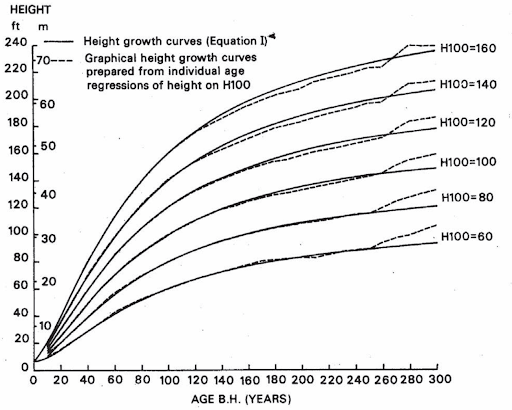
\includegraphics[width=6cm]{Figures/Fig-ageheight.png}
    \caption{Height Growth Curves for Douglas Fir from \cite{five}}
    \label{fig:exampleageheight}
\end{figure}

\subsection{First Iteration}
\subsubsection{Initial Differential Equation}


\begin{equation}
\label{eq:one}
    \frac{\Delta H}{\Delta t} = \text{Total Energy} - \text{Maintenance Energy}
\end{equation}

\begin{equation}
\label{eq:two}
    \frac{\Delta H}{\Delta t} = aL - (bL+cH^3)
\end{equation}

\begin{equation}
\label{eq:three}
\begin{split}
    \frac{\Delta H}{\Delta t} & = (a-b)L - cH^3 \\
    & = kL - cH^3
\end{split}
\end{equation}

\begin{equation}
\label{eq:four}
    \frac{\Delta H}{\Delta t} = d \frac{t}{t+1} - ct
\end{equation}



The variables used are:
\begin{itemize}
\item $H$ - Height in metres
\item $t$ - Time in years
\item $L$ - Leaf Area in $m^2$
\item $a, b, c, d$ - Constants
\item $h_0$ - Initial/Sapling Height in metres
\end{itemize}

The total energy of a tree is related to its total leaf area, L. The rate of growth of the tree is modelled as being directly related to the spare energy it has when the energy needed to maintain itself is deducted from the total energy it has produced. 

Equation \ref{eq:two} shows how we represent total and maintenance energy. The total energy is dependent on leaf area and represented as $aL$. Maintenance energy is comprised of: energy used to maintain the leaves, $bL$, and the trunk, $cH^3$. This is simplified to Equation \ref{eq:three}. This is a nonlinear differential equation and consequently, it is difficult to solve numerically. The differential equation is nonlinear because leaf area and trunk maintenance are functions of the height $H$.  In order to simplify the model and obtain solutions, these values are estimated as functions of time. For trunk maintenance, we can assume height increases indefinitely until the model reaches maximum height, so we replace $cH^3$ with $ct$. As for leaf area, we can use $L = d(\frac{t}{t+1})$ since this function increases somewhat linearly and tends to the constant $d$, which will be the energy produced by the leaves minus the energy used to maintain them. These substitutions construct the simplest iteration of the differential equation model. Solving this numerically produces the solution:
\begin{equation}
\label{eq:five}
    H(t) = h_0 - \frac{ct^2}{2} + dt - d \log(t+1)
\end{equation}

Inputting constants into this solution we can plot the height over the tree’s lifespan. The $h_0$ constant is the initial height of the tree when we start modelling its growth. For simplicity, we start when the tree is just a sapling, or 1m tall. Most of a tree’s trunk is made of dead cells that don’t require much maintenance. For example, the bark of every tree serves to protect itself from diseases and insects but is entirely made up of dead cells \cite{one}. The main ‘living’ component of the trunk is the cambium, which is a thin layer that is responsible for making the trunk thicker \cite{two}. Because so little of the trunk will require maintenance energy we can assume the value of the constant c in this iteration is small; we used a value of $c=0.02$ as an estimate. We adjusted the value of d to produce an appropriate plot, where $d=1.2$.

\begin{figure}[htp]
    \centering
    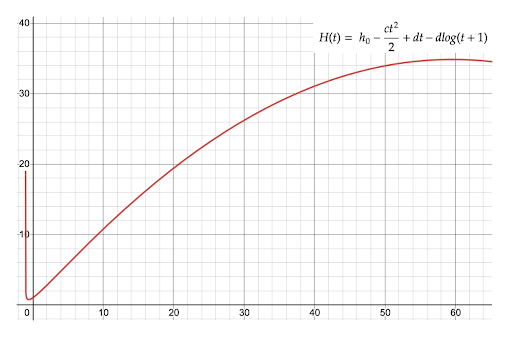
\includegraphics[width=7cm]{Figures/Figure1}
    \caption{Plotted solution of the First Iteration}
    \label{fig:firstsolution}
\end{figure}





\subsubsection{Analysis}

This is the most straightforward model for the height of a Douglas Fir tree. Comparing its solution to actual data shows it sufficiently predicts the average tree’s height and growth over its lifespan to a reasonable degree of accuracy. This first iteration has a growth rate of 58.3cm per year at 30 years of age and similarly, the growth rate of Douglas Fir trees is 61cm per year at the same age. The model also has a maximum height of 34.9m and likewise mature interior Douglas Fir trees reach heights between 30 - 37m on average \cite{three}.

However, this model also has its drawbacks. For instance, instead of settling at its maximum height the change in height becomes negative. This is the result of our assumption that the trunk’s required energy for maintaining itself continues to increase indefinitely. Therefore this model can only be used to project growth up until reaching its maximum height. The model also has approximated that the tree will reach its full height after 57.6 years. This is inaccurate as Douglas Fir trees can continue growing until nearly 200 years old, although they grow at a much slower rate. Additionally, our first iteration estimates the leaf area using a determined value that isn’t based on the height of the tree.


\subsection{Second Iteration}
\subsubsection{Changes}

To improve the first iteration a new technique for modelling the leaf area was introduced and subsequently the energy the tree receives. To model how leaf area changes over the tree’s lifespan a sigmoid function was used which exponentially increases at the beginning and gradually settles on a given constant, $l$. This model was chosen since the leaf area will also grow exponentially when the tree has leaves but very little structure to maintain. The function to calculate leaf area looks like this:

\begin{equation}
\label{eq:six}
    L = \frac{l}{1+e^{-0.1(t-30)}}
\end{equation}

To make this model accurate the value of the leaf area on which it settles needed to be calculated, in other words, the maximum leaf area. This was done by assuming the leaf area can be estimated by the surface area of a cone minus the area of the trunk in contact with the cone. This assumption is made to simplify the calculations because the leaves of a Douglas Fir tree are similar in appearance. The formula for this is:
\begin{equation}
\label{eq:seven}
    l = \pi (R \sqrt{h_{\text{crown}^2 + R^2}} + (R^2 - r^2))
\end{equation}


Where $R$ is the radius of the leaves, $r$ is the radius of the trunk and $h_\text{crown}$ is the depth of the tree’s crown. The crown of the tree is its canopy measured from its first major branches to the top of the tree. To find values to use for this calculation, statistics from a study of 854 harvested Douglas Fir trees across Washington, Oregon and California \cite{four} were used. For the trunk width, the DBH or diameter of the trunk at breast height was used and estimated the crown width as $R$ = 3r. Accordingly, $h_\text{crown}$= 18.1m, $r$ = 1m, $R$ = 3m. This meant the leaf area of a mature Douglas Fir was estimated  to be $4.67\text{m}^2$. The final equation for leaf area is:

\begin{equation}
\label{eq:eight}
    L = \frac{4.67}{1+e^{-0.1(t-30)}}
\end{equation}

\begin{figure}[htp]
    \centering
    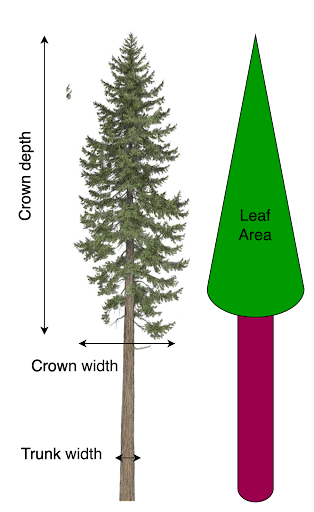
\includegraphics[width=5cm]{Figures/Figure2}
    \caption{Diagram of Tree Measurements used to Calculate Leaf Area\cite{six}}
    \label{fig:treediagram}
\end{figure}

Given the ability to estimate the growth of the tree’s leaf area, the energy produced from it needed to be calculated. Supposing that the average mature fir tree will absorb 25kg of CO$_2$ every year\cite{seven}, the energy it produces each year is approximately 92MJ, assuming that photosynthesis is 100\% efficient. Dividing our annual energy by our max leaf area tells us that leaves produce 19.7MJ per m$^2$ of leaf area. Our equation for total energy produced by the tree, with E$_L$ as annual energy per m$^2$ is as follows:

\begin{equation}
\label{eq:nine}
    \text{Total Energy} = E_L\frac{4.67}{1+e^{-0.1(t-30)}}
\end{equation}

It is assumed the maintenance energy of the tree will eventually equal 92MJ at which point it will stop growing. In order to model the maintenance energy, a function that tends towards the annual energy produced, $A$, was used. This function was chosen because it has an asymptote and increases rapidly. This is similar to how a tree’s maintenance energy grows as it is related to the volume of its crown and trunk.

\begin{equation}
\label{eq:ten}
    \text{Maintenance Energy} = \frac{A}{1+e^{-0.03(t-100)}}
\end{equation}

Combining this with our total energy equation gives us:

\begin{equation}
\label{eq:eleven}
    \frac{dE}{dt} = E_L\frac{4.67}{1+e^{-0.1(t-30)}} - \frac{A}{1+e^{-0.03(t-100)}}
\end{equation}

\begin{equation}
\label{eq:twelve}
    \frac{dH}{dt} = x(E_L\frac{4.67}{1+e^{-0.1(t-30)}} - \frac{A}{1+e^{-0.03(t-100)}})
\end{equation}

\begin{equation}
\label{eq:thirteen}
    \frac{dH}{dt} = 0.005(19.7\frac{4.67}{1+e^{-0.1(t-30)}} - \frac{92}{1+e^{-0.03(t-100)}})
\end{equation}


It is assumed that all the excess energy of the tree is used for growth and that it is directly proportional to growth. $x$ is a constant that takes the value 0.005, it converts the change in energy to the change in height (Figure \ref{fig:2nddiff}).

This was then integrated and a constant of 1m was used for the initial height of the tree, this gave us the graph for height against time (Figure \ref{fig:2ndint}).

\begin{figure}[htp]
    \centering
    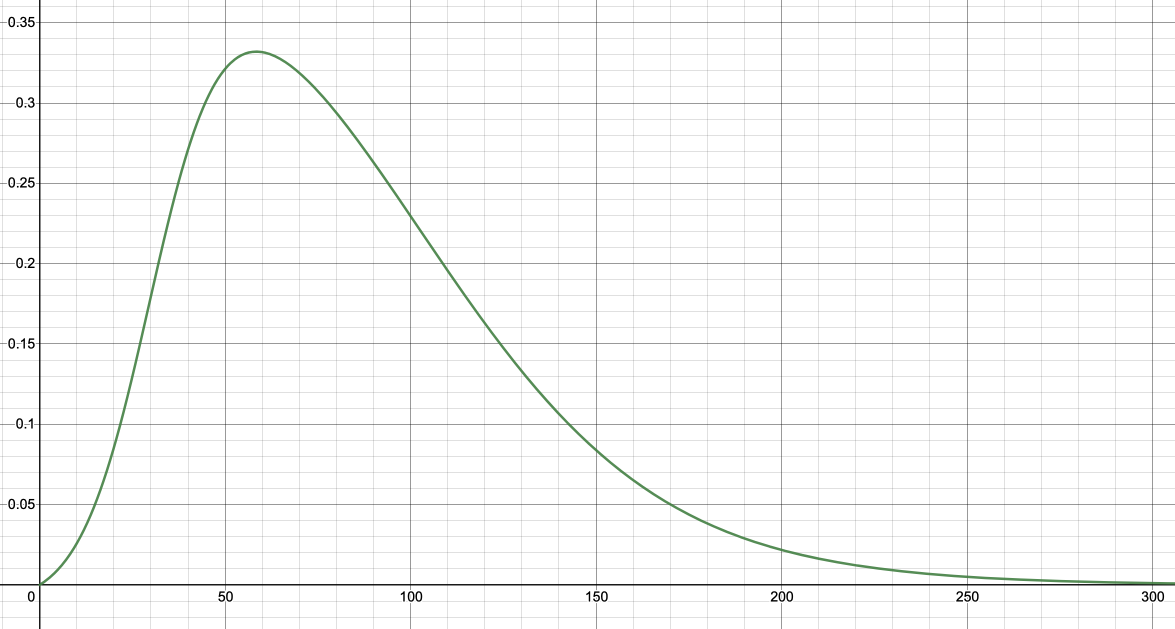
\includegraphics[width=6cm]{Figures/Figure3}
    \caption{Graph of Change in Height/Metres against Time/Years}
    \label{fig:2nddiff}
\end{figure}


\begin{figure}[htp]
    \centering
    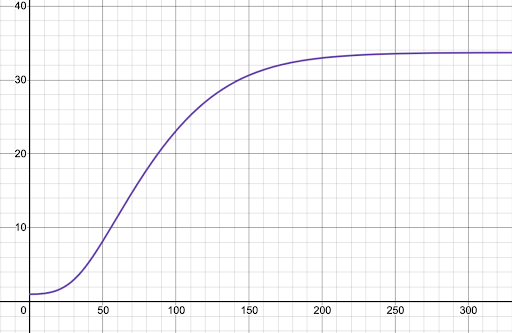
\includegraphics[width=6cm]{Figures/Figure4}
    \caption{Graph of Height/Metres against Time/Years}
    \label{fig:2ndint}
\end{figure}


\subsubsection{Analysis}

Examining our results for our second iteration, the model settles on a maximum height of approximately 34m, and reaches its max height after almost 200 years. This is accurate because Douglas Fir trees can live and continue to grow for hundreds of years, this also improves on the first iteration which suggested the tree reaches maximum height after 57.6 years. The average height of interior Douglas Fir trees reaches heights between 30 - 37m on average \cite{three}, which is within range of  our value of maximum height. Additionally, this model can be used to predict the height accurately late in the tree’s lifespan:


\begin{table}[ht]
\centering
\begin{tabular}{|p{1cm}|p{1.5cm}|p{1.5cm}|p{1.5cm}|}
\hline
Age, years & Modelled height, m & Actual height from study, m & Percentage difference, \% \\ \hline
20  & 1.6  & 5.8  & 113.5 \\ \hline
60  & 11.5 & 16.0 & 32.7  \\ \hline
100 & 23.1 & 23.0 & 0.4   \\ \hline
200 & 33.0 & 31.5 & 4.7   \\ \hline
300 & 33.7 & 35.1 & 4.1   \\ \hline
\end{tabular}
\caption{Comparison of modelled height and statistics from Table 2 in \cite{eight}}
\label{tab:my-table}
\end{table}

This model is unreliable for projecting height early in the tree’s life. Our model has less growth during 10 - 100 years of age than the typical Douglas Fir in \cite{eight}.




%----------------------------------------------------------------------------------------
%	DISCUSSION AND CONCLUSION
%----------------------------------------------------------------------------------------

\section{Discussion and Conclusion}
\subsection{Results}

Our First Iteration was our most rudimentary solution to predicting a Douglas Fir’s height over its lifespan. Despite this method’s simplicity, it accurately predicts the growth rate of interior Douglas Fir trees early in life and their maximum height at maturity. On the other hand, the solution incorrectly projects the tree to reach its maximum height at 57.6 years of age and to decrease in height soon thereafter. In reality, Douglas Fir trees stop growing at approximately 200 years of age \cite{three}. Our results indicate this model is useful for modelling maximum height and initial growth but inaccurate for modelling a tree’s entire growth or lifespan.

Our Second Iteration is an advancement in complexity and accuracy. This model correctly tends toward a growth rate of $\frac{dH}{dT} = 0 $, therefore has a maximum height and remains constant at its maximum. Furthermore, the second iteration describes the maximum height, maturity age and growth rate with adequate accuracy. The maximum height of 34m is average for most Douglas Fir trees and by 200 years of age, its growth rate is almost negligible in both the model and real data. The only disadvantage of this model is that the growth of the tree early in its life is unreliable, however, this model is valid for predicting height 60 years and beyond.

\subsection{Improvements}

To improve our model fewer assumptions could have been made. For example, it is assumed that there were no roots to simplify the model. Including the roots would have a significant impact on the method since roots take large amounts of energy to maintain themselves and to grow. Assuming the tree received all the nutrients and water it needed was another property that was assumed. Factoring this in would lead to growth shifting a lot more due to changing seasons and climate, the growth rate would be greater when rain and sunlight are plentiful. If there was more time the model could have been extended to predict the height of other species rather than just the Douglas Fir. However, species vary greatly in growth and height, so this would be very complicated to implement.





%----------------------------------------------------------------------------------------
%	REFERENCES
%----------------------------------------------------------------------------------------

\begin{thebibliography}{99} % Bibliography - this is intentionally simple in this template

\bibitem[1]{one}
Steve Nix, "How Much of a Tree Is Alive? Understanding Living and Non-Living Tree Cells"
\url{https://www.treehugger.com/how-much-of-tree-is-alive-3967213#}
 
\bibitem[2]{two}
"How A Tree Works!"
\url{https://treescharlotte.org/wp-content/uploads/2013/11/How-A-Tree-Works.pdf}

\bibitem[3]{three}
Average mature height of interior Douglas-fir tree and growth rates  - \url{https://www.srs.fs.usda.gov/pubs/misc/ag_654/volume_1/pseudotsuga/menziesii.htm}

\bibitem[4]{four}
Statistics for Douglas Fir measurements
\url{https://www.fs.fed.us/pnw/pubs/journals/pnw_2009_hummel001.pdf}

\bibitem[5]{five}
Height Growth and Site and Index for Douglas-fir in High-Elevation Forests of the Oregon-Washington Cascades
\url{https://www.fs.fed.us/pnw/olympia/silv/publications/opt/147A_CurtisEtal1974.pdf}

\bibitem[6]{six}
Diagram of Douglas Fir original image source
\url{https://www.conifers.org/pi/Pseudotsuga_menziesii.php}

\bibitem[7]{seven}
Supposing that the average mature fir tree will absorb 25kg of CO2 every year
\url{https://ecotree.green/en/how-much-co2-does-a-tree-absorb}

\bibitem[8]{eight}
Estimates of Site Index and Height Growth for Douglas-Fir in HighElevation Forests of the OregonWashington Cascade Range: Curves and Tables for Field Application
\url{https://www.fs.fed.us/pnw/pubs/pnw_rp378.pdf}

 
\end{thebibliography}

%----------------------------------------------------------------------------------------

\end{document}
